\documentclass[aspectratio=169,hyperref={unicode}]{beamer}

\usetheme{Szeged}
\usecolortheme{beaver}
\usepackage{fontspec}
\usepackage{xcolor}
\usepackage{ulem}
\usepackage{hyperref}
\usepackage[german]{babel}
\usepackage{amssymb} 
\usepackage{tikz} 
\usetikzlibrary{positioning}

\tikzset{set/.style={draw,circle,inner sep=0pt,align=center}}



\title{Info on Generative AI Use}
\author{Rofaïda Rabehi \& Erik Zeiner}
\institute{Fachschaft General \& Computational Linguistics\\ \textbf{University of Tübingen}}
\date{WS 2024/25 \\ Pre-course}

\begin{document}


\frame{\titlepage}



\section{What is Generative AI?}

\begin{frame}
\begin{minipage}{.5\textwidth}
	\textbf{People not in the know like to mix up and misuse:}
  \begin{itemize}
  	\item Artificial Intelligence
  	 \begin{itemize}
  		\item Generative AI
  	\end{itemize}
  	\item Deep learning
  	\item Machine learning
  	\item Large Language Models
  	\item Neural Networks
  	\item ...
  \end{itemize}
\end{minipage}% 
\begin{minipage}{.5\textwidth}
  	\begin{tikzpicture}
\node[set,fill=green!20,text width=7.4cm,label={[below=180pt of rea,text opacity=1]Artificial intelligence}] 
  (ai) at (0,-0.4)  (rea) {};
\node[set,fill=blue!20,text width=5cm,label={[below=114pt of rea,text opacity=1]Machine learning}] 
  (nat) at (0,-0.4)  (rea) {};
\node[set,fill=red!20,text width=3.5cm,label={[below=66pt of int]Deep learning}] 
  (int) at (0,-0.2)  {};
\node[set,fill=olive!20,text width=1.5cm] (nat) at (0,0) {LLMs};
\end{tikzpicture}
\end{minipage}
	
\end{frame}

\begin{frame}{How Can Machines (and LLMs) Learn?}
\begin{center}
	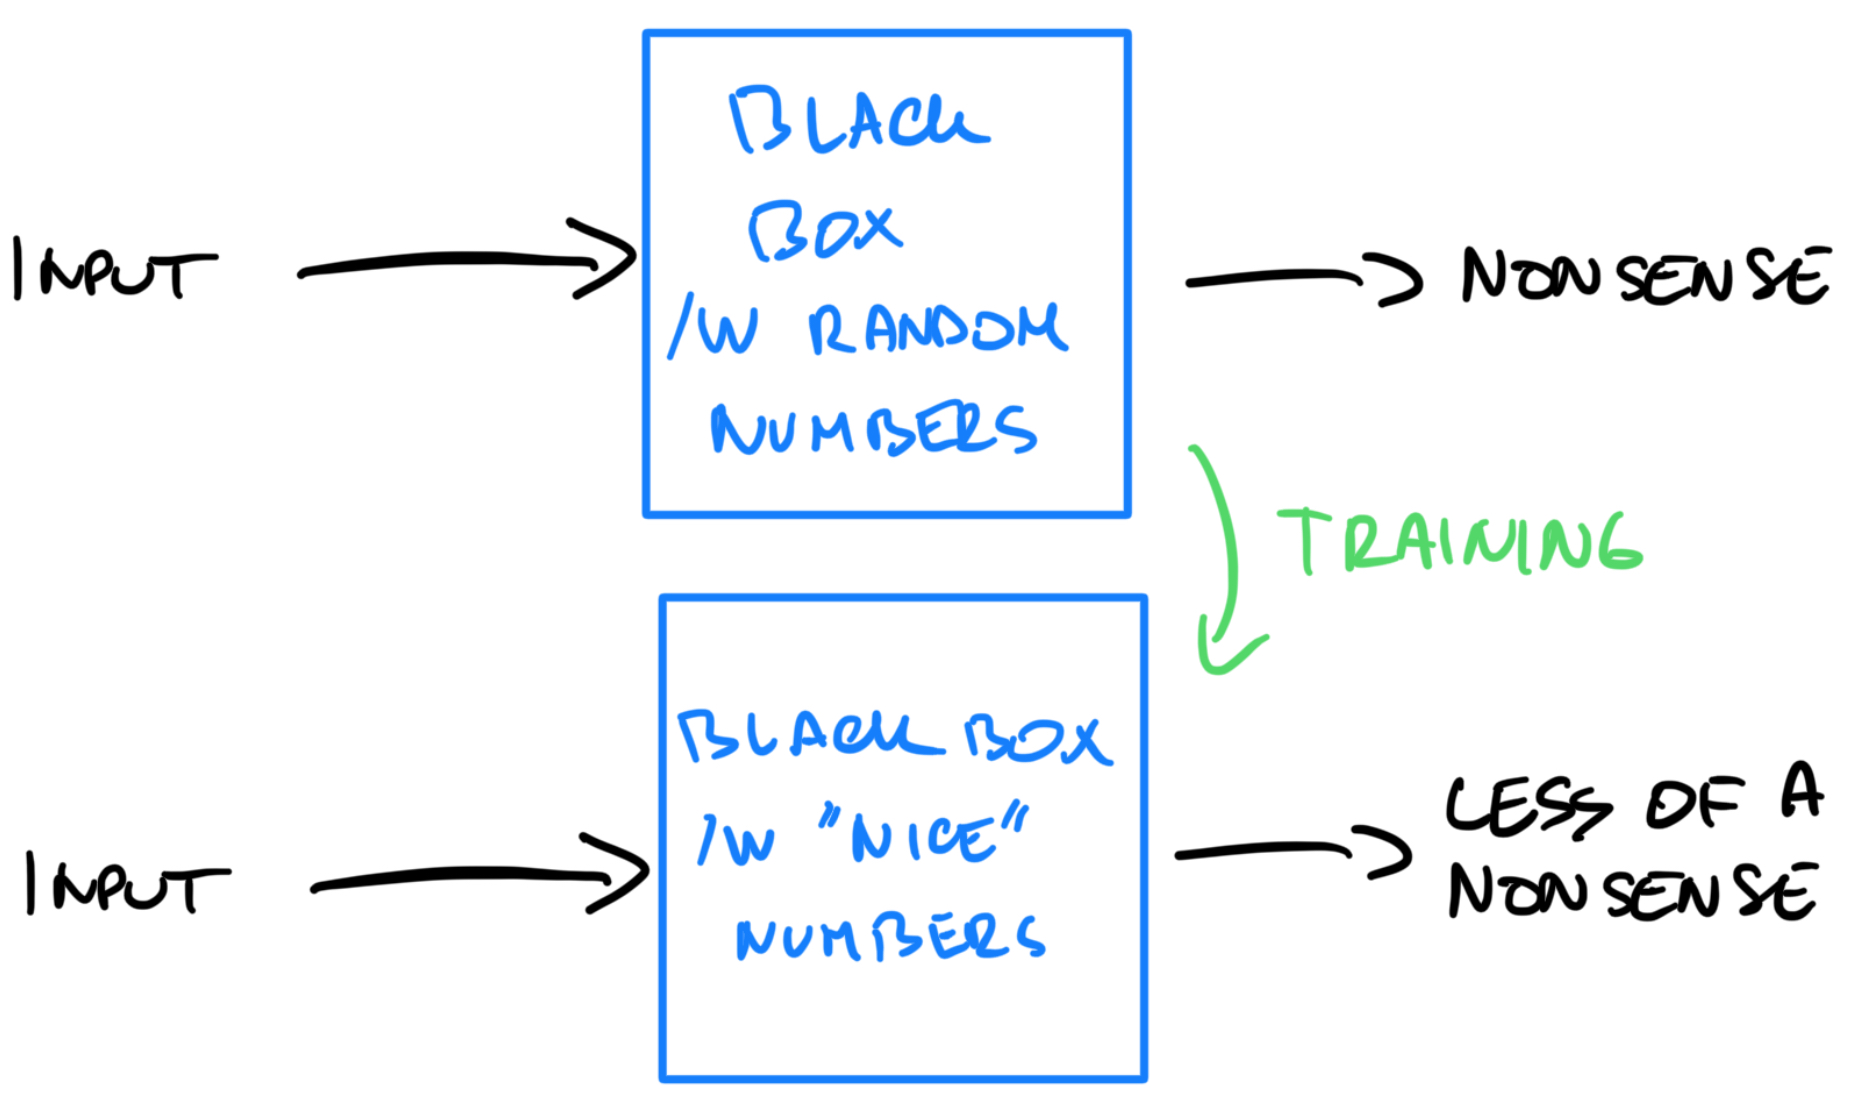
\includegraphics[scale=0.3]{training.jpg}
\end{center}
\end{frame}

\begin{frame}{Large Language Models}
\begin{alertblock}{Why are they models?}
attempt to ''do language'' like ''we would''
\end{alertblock}

\begin{alertblock}{Why language specifically?}
trained on natural language, good for tasks such as modelling, translation, summarisation, classification,...
\end{alertblock}

\begin{alertblock}{What makes them large?}
learned knowledge about language and the world from vast amounts of text
\end{alertblock}

\end{frame}

\section{What is it good for?}

\begin{frame}
	rofi
	
	(suggestion: helper with the mundane when you can verify the results yourself )
\end{frame}

\section{What are the limitations?}

\begin{frame}{Inherent limitations}
\begin{alertblock}{Bias}
If its in the training data, it may appear in the output\\
toxic language, gender bias, race bias,...
\end{alertblock}

\begin{alertblock}{Hallucinations}
prone to make things up - text is coherent but false	
\end{alertblock}

\begin{alertblock}{Copyright/Privacy Issues}
Where did its knowledge come from?

Where did my knowledge come from?
	
\end{alertblock}

\end{frame}

\begin{frame}{When things don't go as expected...}
	example of limitations translation
\end{frame}

\begin{frame}{When things don't go as expected...}
	examp                                                                                                                                                                                                                                                                                                                                                                                                                                                                                                                                                                                                                                                                                                                                                                                                                                                                                                                                                                                                                                                                                                                                                                                                                                                                                                                                                                                                                                                                                                                                                                                                                                                                                                                                                                                                               le of limitations - cl related
\end{frame}

\section{Should you (not) use it for university work?}

\begin{frame}{Stance of the Universtity}
	rofi
\end{frame}

\begin{frame}{Recommendations}
	rofi
\end{frame}


\begin{frame}
\begin{center}

\textbf{Think critically, like a computational linguist}

---

\textbf{Don't rely on it}

---

\textbf{Use with care and consideration}


\vspace{1em}

\begin{minipage}{0.4\textwidth}
\centering
    
\includegraphics[width=0.5\textwidth]{QRtemplate_5.png}
  \end{minipage}
  \hfill
  \begin{minipage}{0.4\textwidth}
  \centering
    
\includegraphics[width=0.5\textwidth]{QRtemplate_4.png}
  \end{minipage}
\end{center}
\end{frame}
\end{document}